\subsection{Rate--Distortion Comparison: the Intrinsic Gap and the Critical Overhead}
\label{sec:rd_main}

Three quantities carry the result of this paper. They are reported in an
order such that no assumption is introduced before it is needed. The first
is the intrinsic HEALPix/UTM size ratio at equal reconstruction error, with
no overhead assigned to either product ($\gamma=1$); it is a property of the
two grids and of the transfer that populated one of them. The second is the
same ratio read as a decision threshold, the distortion-dependent
\emph{critical overhead} $\gamma_\star(e)$, defined as the native-product
overhead above which the carrier becomes the smaller representation at error
$e$. This is the general result, and it is a curve rather than a verdict.
The third is one point on that curve, an illustrative $30\%$ granule
overhead ($\gamma_{\mathrm{tile}}=1.30$), reported in
Section~\ref{sec:rd_illustrative} because a concrete operating point is
useful, and reported after the curve because it is not the result.

At $\gamma=1$, native UTM is intrinsically the more compressible
representation over the whole tested RMSE range, by a margin that decreases
monotonically as the target loosens: $+106\%$, $+94\%$, $+60\%$, $+25\%$ and
$+6\%$ from $10^{-4}$ to $10^{-2}$.

Restating this gap as
$\gamma_\star(e)=S_{\mathrm{HPX}}(e)/S_{\mathrm{UTM,crop}}(e)$ is an
accounting identity rather than an explanation. The change of sign at
$\gamma=\gamma_\star$ is tautological and says nothing about why the gap
narrows with distortion; what the identity provides is a threshold that a
product designer can compare with a measured overhead.
Table~\ref{tab:gamma_continuous} reports $\gamma_\star$ at every target. It
decreases from $2.06$ to $1.06$ and reaches $1.25$ at $3\times10^{-3}$, just
below the illustrative $1.30$, which is why the measured ratio at that
target is $0.96$, the closest to parity of any target. At the three tightest
targets $\gamma_\star$ ranges from $1.60$ to $2.06$, overheads that we are
not aware of any measurement supporting, and at the tightest target native
UTM remains ahead for three quarters of the regions even at $\gamma=2$. At
the loosest targets $\gamma_\star$ falls to $1.06$--$1.25$, so that a native
product organised with less overhead than assumed here would restore the
advantage of UTM there as well. The value of $\gamma_\star$ has not been
recomputed for the matched-budget protocol, which would require repeating
the budget interpolation at $\gamma=1$ (Section~\ref{sec:limitations}).

\begin{table*}[t]
\centering
\caption{The verdict over a continuous range of the overhead ratio $\gamma=\gamma_{\mathrm{UTM}}/\gamma_{\mathrm{HPX}}$}
\label{tab:gamma_continuous}
\footnotesize
\begin{tabular}{lrrlrrrl}
\toprule
Target RMSE & $n$ & $\gamma_\star$ & IQR & \multicolumn{3}{c}{HPX smaller (\% of regions)} & Inconclusive \\
\cmidrule(lr){5-7}
 & & median & & $\gamma{=}1$ & $\gamma{=}1.3$ & $\gamma{=}2$ & $\gamma$ range \\
\midrule
$10^{-4}$ & 40 & 2.27 & [2.18, 2.37] & 0 & 2 & 10 & $2.21$--$2.33$ \\
$3\times10^{-4}$ & 40 & 2.18 & [2.00, 2.28] & 2 & 2 & 25 & $2.06$--$2.21$ \\
$10^{-3}$ & 39 & 1.82 & [1.48, 2.02] & 8 & 21 & 72 & $1.54$--$1.92$ \\
$3\times10^{-3}$ & 37 & 1.61 & [1.18, 1.84] & 11 & 32 & 86 & $1.37$--$1.71$ \\
$10^{-2}$ & 33 & 1.53 & [1.25, 1.98] & 12 & 33 & 76 & $1.33$--$1.72$ \\
\bottomrule
\end{tabular}
\vspace{3pt}
\begin{minipage}{\textwidth}
\footnotesize
Each region's critical overhead $\gamma_\star$ is the value at which the two representations reach equal compressed size for that region, so HEALPix is the smaller of the two exactly where $\gamma\ge\gamma_\star$; the win columns are the fraction of the 40 regions satisfying that at three illustrative values. \emph{Inconclusive} is the range of $\gamma$ over which the paired signed-rank test does not separate the two grids at the $5\%$ level. No value of $\gamma$ is privileged: the table maps an assumption a reader may hold to the conclusion it implies.
\end{minipage}
\end{table*}


\begin{figure}[t]
\centering
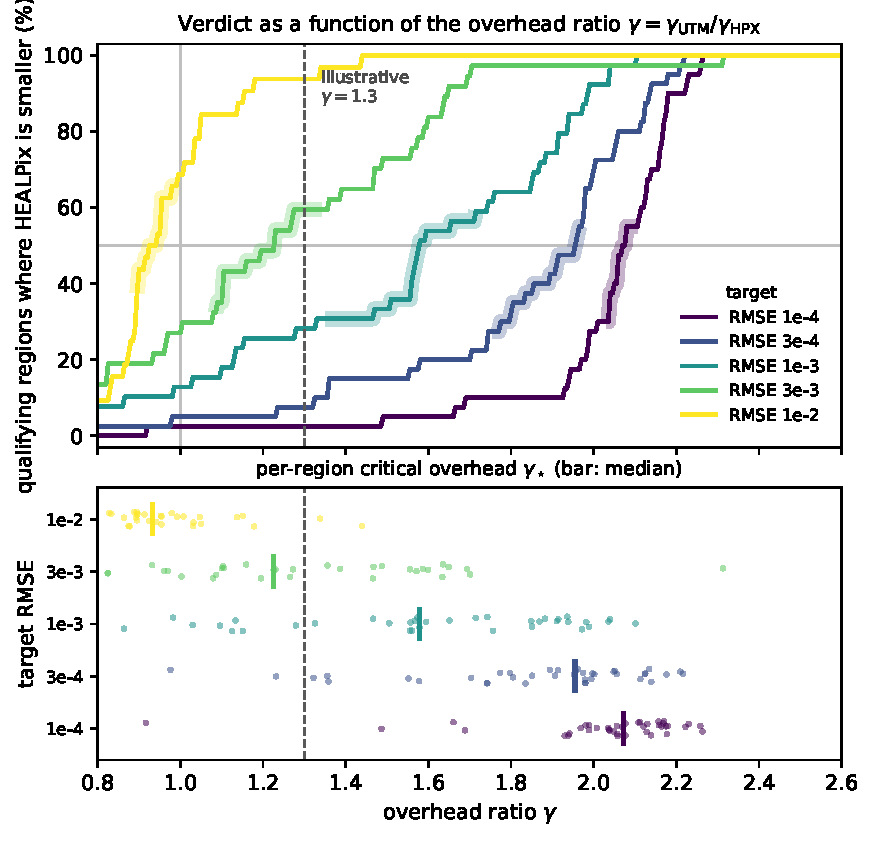
\includegraphics[width=\columnwidth]{figures/fig_verdict_vs_gamma}
\caption{The verdict over a continuous range of the overhead ratio
$\gamma=\gamma_{\mathrm{UTM}}/\gamma_{\mathrm{HPX}}$, rather than at one assumed
value. Top: the fraction of the 40 regions for which HEALPix is the smaller
representation, per RMSE target; the thickened stretch of each curve is where
the paired signed-rank test does not separate the two grids at the $5\%$ level.
Bottom: the per-region critical overhead $\gamma_\star$ behind those curves, one
point per region, the bar marking the median. The dashed line marks the
illustrative $\gamma_{\mathrm{tile}}=1.30$ used elsewhere in this paper; it is
marked, not privileged.}
\label{fig:verdict_vs_gamma}
\end{figure}

Because the overhead enters as a single multiplicative factor, every
statement about it is a function of one per-region quantity. The intrinsic
ratio of a region is its $\gamma_\star$; HEALPix is the smaller
representation exactly where $\gamma\ge\gamma_\star$, and the paired test at
overhead $\gamma$ is the signed-rank test on $\log(\gamma_\star/\gamma)$.
Verdict, significance and spread are therefore all read from the empirical
distribution of $\gamma_\star$ (Fig.~\ref{fig:verdict_vs_gamma}). Reading
$\gamma$ in this way also removes an asymmetry. With an overhead
$\gamma_{\mathrm{HPX}}$ on the carrier and $\gamma_{\mathrm{UTM}}$ on the
native product, the only parameter that matters is the ratio
$\gamma=\gamma_{\mathrm{UTM}}/\gamma_{\mathrm{HPX}}$, which is why the figure
extends below $1$: there the carrier carries the heavier container, and a
fifth to a third of the regions already have their critical overhead in
that range at the looser targets. One component of $\gamma$ is measurable,
and Appendix~\ref{app:container} measures it: the container format accounts
for at most half a percent on either side, so that a $30\%$ overhead
describes granule geometry (padding, overlap, per-granule metadata), a
property of a product layout, which is why it is carried as a parameter.

The table shows that no single summary statement is available. A reader
who assumes no overhead ($\gamma=1$) finds HEALPix smaller for
$2\%$ to $35\%$ of the regions depending on the target; one who accepts
the illustrative $1.30$ finds $2\%$ to $78\%$; one who assumes that the
native layout costs twice what the carrier does finds $28\%$ to $98\%$.
Only at the
tightest target is the answer robust over the whole plausible range. Each
target also has a band of $\gamma$, narrow at the extremes and
$1.38$--$1.73$ at $10^{-3}$, within which the two grids cannot be separated
at all; a reader whose product falls in that band should draw no conclusion
from this comparison rather than read off a ratio.
